%%
% Please see https://bitbucket.org/rivanvx/beamer/wiki/Home for obtaining beamer.
%%
%\documentclass[11pt,aspectratio=169]{beamer}
%\documentclass[11pt,aspectratio=169,xcolor={dvipsnames}]{beamer}

\documentclass[11pt,aspectratio=169,xcolor={dvipsnames},hyperref={pdftex,pdfpagemode=UseNone,hidelinks,pdfdisplaydoctitle=true},usepdftitle=false]{beamer}
\usepackage{presentation}


\title{Lecture 12: Bank Runs}
\author{Juan Herre\~{n}o\\UCSD}
\date{2026}

% Enter presentation title to populate PDF metadata:
\newcommand{\Cov}{\text{Cov}_\lambda}
\newcommand{\El}{\mathbb{E}_\lambda}
\newcommand{\mm}{\text{{\fontfamily{qzc}\selectfont m}}}
\usepackage{cancel}
\usepackage{booktabs}
\begin{document}

\maketitle




\begin{frame}{Financial Crises}
\begin{itemize}
	\itemsep1em 
	\item Financial crises have been common over the past 400 years
	\item Come in different flavors:
	\begin{itemize}
		\item Banking crises
		\item Currency crises
		\item Sovereign debt crises
	\end{itemize}
	\item Often associated with (the cause of?) major recessions/depressions
	\begin{itemize}
		\item Great Depression, Great Recession
		\item Sweden 91, Mexico 94, Thailand/Korea/etc. 97, Argentina 01, etc.
	\end{itemize}
\end{itemize}
\end{frame}


\begin{frame}{Suddenness of Financial Crises}
\begin{itemize}
	\itemsep1em 
	\item Financial crises often occur suddenly 
	\begin{itemize}
		\item Panics
		\item Speculative attacks
	\end{itemize}
	\item Two views:
	\begin{itemize}
		\item Inevitable consequence of fundamental problems \\ (e.g., bank solvency problem, unsustainable government policy)
		\item Self-fulfilling panics \\ (i.e., multiple equilibria events that need never occur) 
	\end{itemize}
\end{itemize}
\end{frame}


\begin{frame}{Diamond-Dybvig Model}
Key Elements:
\begin{itemize}
	\itemsep1em 
	\item A theory of \textbf{maturity mismatch} in banking: {\color{gray}{banks lend long duration, borrow short duration}}
	\item A model of \textbf{liquidity preference} by consumers: {\color{gray}{Some consumers prefer callable deposits}}
	\item An explanation for \textbf{bank runs} as self-fulfilling panics 
\end{itemize}
\vspace{15pt}
{\small Seminar papers: Diamond and Dybvig (1983) and Bryant (1980)}

\vspace{10pt}
{\small My exposition follows Allen and Gale (2007, ch. 3)}
\end{frame}



\begin{frame}{The Liquidity Problem}
\begin{itemize}
	\itemsep1em 
	\item Three dates: $t = 0, 1, 2$
	\item Two assets:
	\begin{itemize}
		\item Liquid asset: Invest 1 unit at $t$ and get 1 unit at $t+1$ (0 return)
		\item Illiquid asset: Invest 1 unit at $t=0$, get $R>1$ units at $t=2$ or $r<1$ at $t=1$ 
	\end{itemize}
	\item Intuitively:
	\begin{itemize}
		\item Selling assets as a solution to liability issues on the balance sheet (can liquidate illiquid assets)
		\item Illiquid asset is a project that is costly to liquidate before it is complete ($r< 1 < R$)
		\item Captures the possibility of ``fire sales''
		\item Makes liability problems more painful, creating net worth losses (liquidating illiquid assets generates losses)
	\end{itemize} 
\end{itemize}
\end{frame}


\begin{frame}{The Liquidity Problem}
\begin{itemize}
	\itemsep1em 
	\item Continuum of households
	\item Each has endowment of 1 at $t=0$ and 0 afterwards
	\item Subject to random time preference shocks realized after period 0
	\begin{itemize}
		\item Value consumption only at $t=1$ with probability $\lambda$
		\item Value consumption only at $t=2$ with probability $1-\lambda$
		\item Extreme versions of shocks to \textbf{marginal utility}
	\end{itemize}
	\item Utility function:
	\[ u(c_1,c_2) = \left\{ \begin{array}{lll}
	U(c_1) & \text{with prob.} & \lambda \\
	U(c_2) & \text{with prob.} & 1-\lambda 
	\end{array} \right. \] 
\end{itemize}
\end{frame}


\begin{frame}{The Liquidity Problem}
\begin{itemize}
	\itemsep1em 
	\item If household knew at $t=0$ that it was an ...
	\begin{itemize}
		\item Early consumer: It would invest in the liquid (short) asset
		\item Late consumer: It would invest in the illiquid (long) asset  
	\end{itemize}
	\item Problem is that it doesn't know!
	\item Any investment strategy will yield regret in some state of the world
\end{itemize}
\end{frame}


\begin{frame}{Autarky}
\begin{itemize}
	\itemsep1em 
	\item Household must invest at $t=0$ but cannot retrade later \\ (i.e., no trading markets at $t=1$)
	\item But can receive payment in t=1 and hold it to t=2
	\item If hh invests a fraction $\theta$ in the short asset
	\item Expected utility is then (assuming $r=0$ for simplicity)
	\[ \lambda U(\theta) + (1-\lambda)U(\theta + (1-\theta)R) \]
	\item If interior, optimal value of $\theta$ satisfies
	\[\lambda U'(\theta) + (1-\lambda) U'(\theta + (1-\theta)R)(1-R) = 0 \] 
\end{itemize}
\end{frame}


\begin{frame}{Autarky}
\begin{itemize}
	\itemsep1em 
	\item With $U(C) = \log C$, this becomes
	\[ \frac{\lambda}{\theta} + \frac{1-\lambda}{\theta + (1-\theta)R}(1-R) = 0 \]
	or 
	\[ \theta = \frac{R}{R-1} \lambda \] 
	\item For reasonable values of $R$, most wealth in short asset \\ e.g., with $R = 1.2$, $R/(R-1) = 6$.
	\item Liquidity problem prevents autarky household from taking advantage of high returns on long-term projects
\end{itemize}
\end{frame}


\begin{frame}{Equilibrium with Trading at $t=1$}
\begin{itemize}
	\itemsep1em 
	\item Households can trade long and short assets at $t=1$ \\ (but no state-contingent assets at $t=0$)
	\item No asset in period $t=0$ that pays only if you are an early (or late) consumer
	\item Let's use $P$ to denote the price of long assets at $t=1$ 
	\pause
	\item \textbf{Result}: The price of long asset at $t=1$ must be $P=1$
	\begin{itemize}
		\item If $P > 1$: Long asset dominates short asset at $t=0$. No one buys short asset at $t=0$. At $t=1$, early consumers offer long asset for sale, but no buyers. Price collapses to $P = 0$. Contradiction.
		\item If $P < 1$: Short asset dominates long asset at $t=0$. No one buys long asset at $t=0$. At $t=1$, late consumers try to buy long asset to realize a return of $R/P > R$, but no sellers. Price bid up to $P = R$. Contradiction. 
	\end{itemize}

\end{itemize}
\end{frame}


\begin{frame}{Equilibrium with Trading at $t=1$}
\begin{itemize}
	\item At $t=0$, household invests in $x$ units of long asset and $y$ units of short asset with
	\[ x + y = 1 \] 
	\item If early consumer: Sells long assets at $t=1$ and consumes
	\[c_1 = y + Px = y + x = 1\]
	\item If late consumer: Buys long assets at $t=1$ and consumes
	\[c_2 = (x + \frac{y}{P})R = (x+y)R = R \] 
	\item Expected utility
	\[ \lambda U(1) + (1-\lambda)U(R) \] 
	\item Note that there is not perfect insurance. $c_2 > c_1$.
\end{itemize}
\end{frame}


\begin{frame}
\begin{figure}
	\centering
	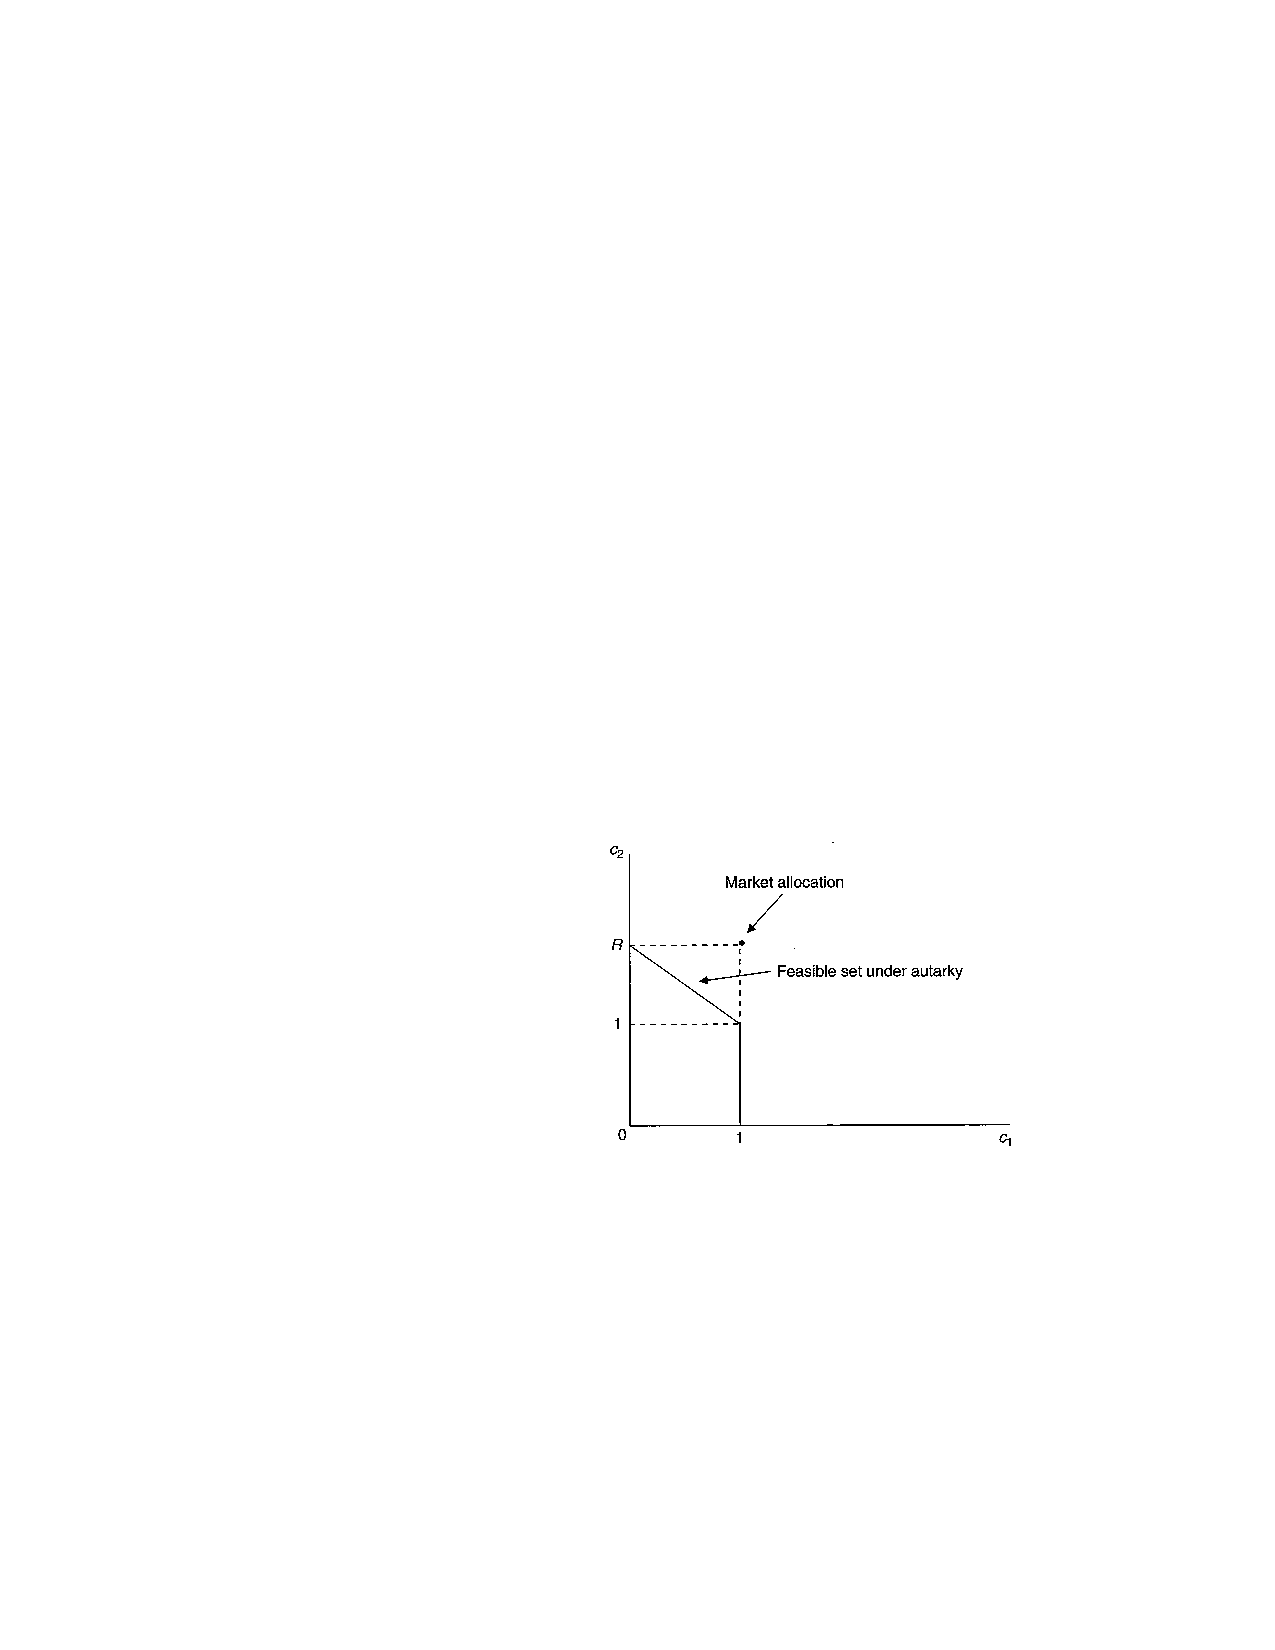
\includegraphics[height=0.9 \textheight]{FiguresTables/AllenGale2007Figure31.pdf}
\end{figure}
\vspace{-3mm}
{\scriptsize Source: Allen and Gale (2007)}
\end{frame}


\begin{frame}{Efficient Outcome}
\begin{itemize}
	\itemsep1em 
	\item Suppose central planner chooses investment and levels of consumption for early and late consumers to maximize household expected utility
	\item Chooses $y$ to maximize
	\[\lambda U\left( \frac{y}{\lambda} \right) + (1-\lambda)U \left( \frac{R(1-y)}{1-\lambda} \right) \]
	\item If solution in interior, must satisfy
	\[ U' \left( \frac{y}{\lambda} \right) - U' \left( \frac{R(1-y)}{1-\lambda} \right) R = 0 \]
	or 
	\[ U'(c_1) = U'(c_2)R \]
	where we use $c_1 = y/\lambda$ and $c_2 = Rx/(1-\lambda)$  
	\item Early consumer get $c_1$, so consumption per capita in $t=1$ is $\lambda c_1$
\end{itemize}
\end{frame}


\begin{frame}{Inefficiency of Trading Equilibrium}
\begin{itemize}
	\item Suppose 
	\[ U(c) = \frac{1}{1-\sigma} c^{1-\sigma}  \]
	\item Optimality condition becomes
	\[ \left( \frac{c_2}{c_1} \right)^{\sigma} = R \]
	\item Equilibrium with trading at $t=1$ has $c_1 = 1$ and $c_2 = R$
	\item Replace the allocation with trading
	\[ R^{\sigma} = R \]
	which only holds for $\sigma = 1$ (log utility case)
\end{itemize}
\end{frame}


\begin{frame}
\begin{figure}
	\centering
	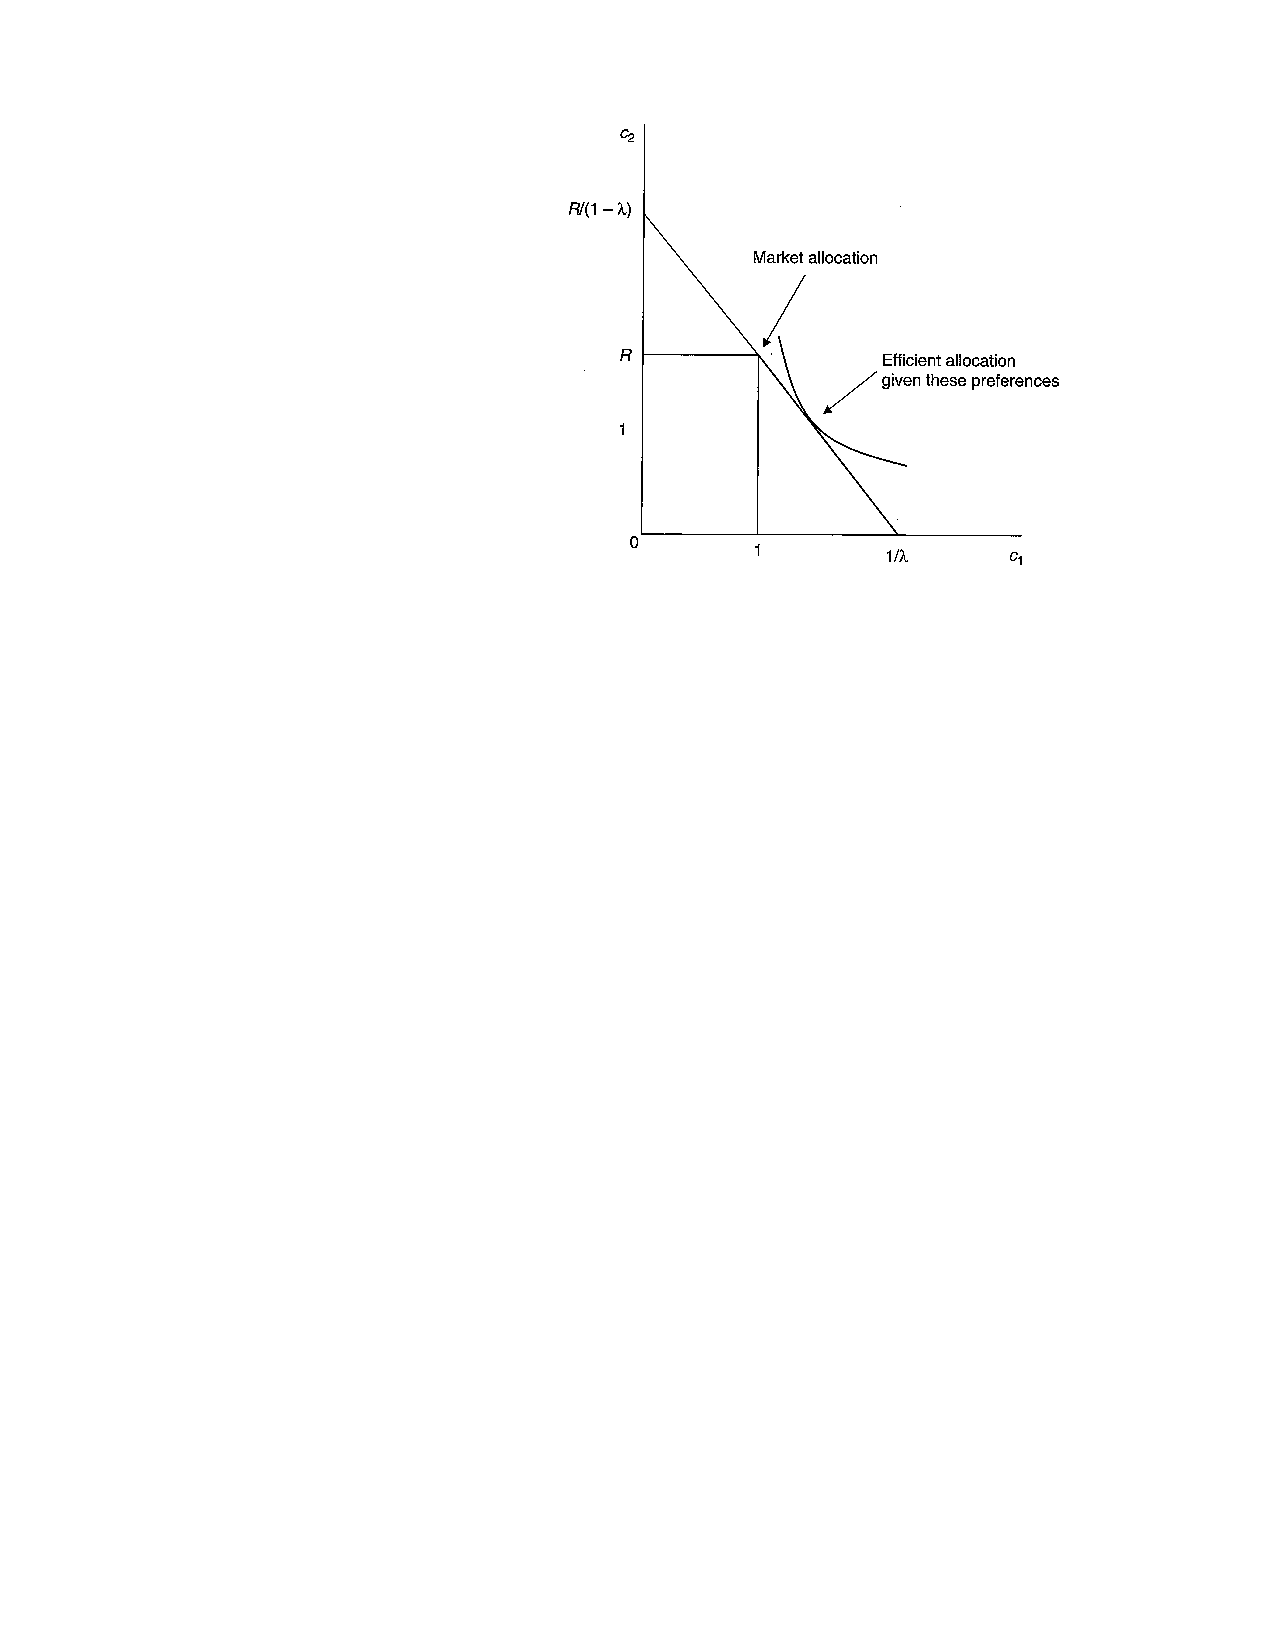
\includegraphics[height=0.9 \textheight]{FiguresTables/AllenGale2007Figure32.pdf}
\end{figure}
\vspace{-3mm}
{\scriptsize Source: Allen and Gale (2007)}
\end{frame}


\begin{frame}{Inefficiency of Trading Equilibrium}
\begin{itemize}
	\itemsep1em 
	\item In trading equilibrium $c_1 = 1 < R = c_2$
	\item In efficient equilibrium $U'(c_1) = RU'(c_2)$. So, $c_1 < c_2$
	\item Consumption stream risky in both cases
	\item When does efficient equilibrium provide more liquidity insurance \\ than trading equilibrium? ($c_2^e/c_1^e < c_2^m / c_1^m$)
	\begin{itemize}
		\item When $\sigma > 1$ (agent more risk averse than log-utility)
	\end{itemize}
	\item When $\sigma < 1$, trading equilibrium provides too much liquidity
	\begin{itemize}
		\item Providing liquidity insurance is expensive
		\item Short asset has low return
	\end{itemize}
\end{itemize}
\end{frame}


\begin{frame}{Banking Solution}
\begin{itemize}
	\itemsep1em 
	\item Large banks:
	\begin{itemize}
		\item Take deposits: Take in 1 at $t=0$, give back $c_1$ at $t=1$ or $c_2$ at $t=2$
		\item Invest in a portfolio (x,y) of long and short assets
	\end{itemize}
	\item Free entry forces banks to maximize household utility (zero profits)
	\item Banking solution same as central planning solution!
	\begin{itemize}
		\item Banks face no risk since they are large
		\item Able to fully diversify liquidity risk of households
	\end{itemize}
	\item One wrinkle: If banks don't observe household type, \\ deposit contract must be \textbf{incentive compatible}  
\end{itemize}
\end{frame}


\begin{frame}{Incentive Compatibility}
\begin{itemize}
	\itemsep1em 
	\item Early consumers won't misrepresent themselves as late consumers
	\begin{itemize}
		\item Would result in zero consumption at time 1
	\end{itemize}
	\item Late consumer could pretend to be early consumer, receive $c_1$ at $t=1$, store it until $t=2$ using short asset
	\item Deposit contract is incentive compatible if
	\[ c_1 \leq c_2 \]
	\item This is the case, as we have seen above
\end{itemize}
\end{frame}


\begin{frame}{Banking in Diamond-Dybvig Model}
\begin{itemize}
	\itemsep1em 
	\item Model of maturity mismatch
	\begin{itemize}
		\item Bank assets are less liquid than bank liabilities
	\end{itemize}
	\item Model of liquidity preference
	\begin{itemize}
		\item Why are bank liabilities so liquid?
		\item Liquidity shock model provides a theory for this
	\end{itemize}
	\item Banks as intermediaries
	\begin{itemize}
		\item Facilitates investment in high return illiquid assets
		\item Provide households with insurance against liquidity shocks
		\item Depositor does better than in autarky or trading equilibrium
	\end{itemize}
\end{itemize}
\end{frame}


\begin{frame}{Bank Runs}
\begin{itemize}
	\itemsep1em 
	\item Let's now consider the case where $0 < r < 1$
	\begin{itemize}
		\item I.e., long asset can be liquidated for $0 < r < 1$ at $t=1$  
	\end{itemize}
	\item Bank must liquidate assets to meet demand for withdrawals at $t=1$
	\item Depositors arrive at teller to withdraw one after another in random order \\ (sequential service constraint)
\end{itemize}
\end{frame}


\begin{frame}{Bank Runs}
\begin{itemize}
	\itemsep1em 
	\item If everyone runs, bank can only pay out
	\[ rx + y < 1 \] 
	\item If
	\[ rx+y < c_1 \] \vspace{-15pt}
	\begin{itemize}
		\item bank will run out of resources before all depositors have been paid
		\item Some depositors that run will get nothing 
		\item Depositors have incentives to run if everybody is running
	\end{itemize}
	\item In this case, a bank run equilibrium exists
\end{itemize}
\end{frame}


\begin{frame}{Bank Runs}
\begin{figure}
	\centering
	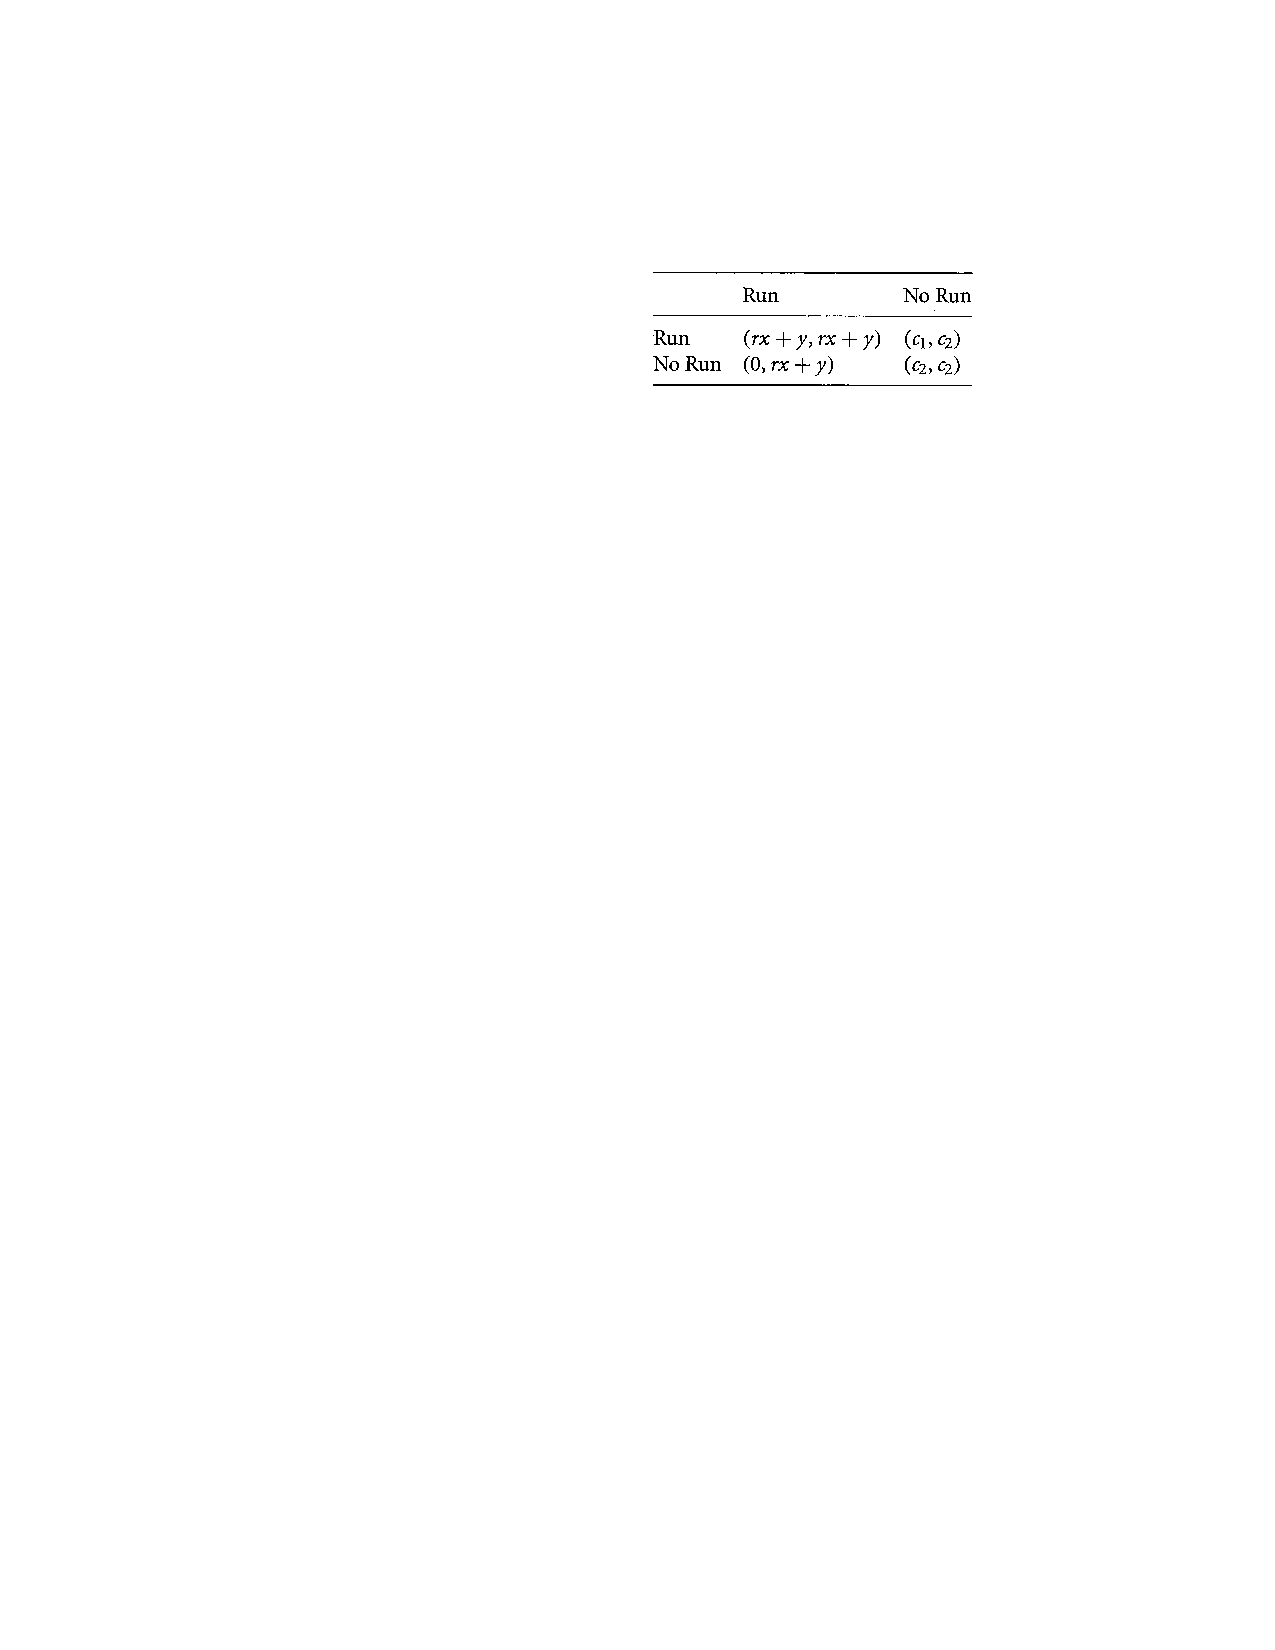
\includegraphics[height=0.4 \textheight]{FiguresTables/AllenGale2007Table.pdf}
\end{figure}
\vspace{-5mm}
\begin{itemize}
	\item Rows: Strategy of depositor A (late consumer)
	\item Columns: Strategy of all other late consumers
	\item Payoffs:
	\begin{itemize}
		\item First entry: Payoff of a depositor A (late consumer)
		\item Second entry: Payoff of all other late consumers 
	\end{itemize}
\end{itemize}
\end{frame}


\begin{frame}{Bank Runs}
\begin{itemize}
	\itemsep1em 
	\item Run equilibrium is a pure coordination problem
	\item Bank has no ``fundamental'' problem
	\item If no one runs, everything would be fine
	\item Pure waste. Completely inefficient. 
	\item Example of multiple equilibria due to strong strategic complementarity 
\end{itemize}
\end{frame}


\begin{frame}{Fundamental Fragility of Banks}
\begin{itemize}
	\itemsep1em 
	\item Even strong banks are fragile to runs
	\item Arises due to maturity mismatch of bank assets and liabilities
	\item Maturity mismatch is due to:
	\begin{itemize}
		\item Household demand for liquidity (due to liquidity shocks)
		\item Desire to take advantage of high return on illiquid asset
	\end{itemize}
\end{itemize}
\end{frame}




\begin{frame}{Preventing Bank Runs}
How can we prevent bank runs? \pause 
\begin{itemize}
	\item Suspension of Convertibility (from deposits to cash)
	\begin{itemize}
		\item Bank refuses to honor depositor withdrawal requests (in the model: in T=1)
		\item Common in US prior to founding of the Federal Reserve
		\item If bank commits to suspend convertibility before it needs to engage in costly liquidation of long asset, late consumers have no need to run
		\item Eliminates the run equilibrium
		\item But if there is uncertainty about how many withdrawals constitute a run, i.e., uncertainty about $\lambda$, this might not work
		\item Big costs of suspension in this case for those that need liquidity
		\item And impair the supply of deposits, and of credit as a consequence
	\end{itemize}
\end{itemize}
\end{frame}



\begin{frame}{Preventing Bank Runs}
\begin{itemize}
	\addtocounter{enumi}{1}
	\item Deposit insurance
	\begin{itemize}
		\item If government insures that late consumers will get there money back \\ even if bank fails, late consumers no long have an incentive to run
		\item This eliminates the run equilibrium
		\item But insured depositors will not monitor the bank. This invites moral hazard on the part of the bank {\small (Calomires-Kahn 91)}
		\item Also, deposit insurance doesn't cover wholesale repo financing  
	\end{itemize}
\end{itemize}
\end{frame}



\begin{frame}{Preventing Bank Runs}
\begin{itemize}
	\addtocounter{enumi}{2}
	\item Lender of Last Resort
	\begin{itemize}
		\item The central bank commits to lend enough to the bank so that it can honor deposits withdrawn at $t=1$ without liquidating the long asset
		\item Late consumers can rest easy. No run equilibrium.
		\item But is the crisis a liquidity or solvency crisis?
		\item Bagehot's rule:
		\begin{itemize}
			\item Lend freely, but at a penalty rate, and against good collateral
		\end{itemize}
		\item Tricky issue: How good is the collateral? \\ Difficult to value in the midst of a crisis
	\end{itemize}
\end{itemize}
\end{frame}


\end{document}




